\documentclass{article}
\usepackage{graphicx} % Required for inserting images
\usepackage{amsmath}
\usepackage{amssymb} % used for math symbols
\usepackage{mathtools}
\usepackage{enumitem}
\usepackage{wasysym}
\usepackage{float}


\title{Computer Grafik Blatt 7}
\date{June 2023}

\begin{document}

\maketitle

\section*{Aufgabe 1.}

\subsection*{(a)}

$T(0.3,0.9)= T(0,1) = 100$ da die Stelle in dem Pixel $T(0,1)$ liegt. Wir gehen hier davon aus, das die Pixel durch ihren Mittelpunkt gegeben sind.


\subsection*{(b)}

\begin{align*}
    T(0,0.9) &= 0.1\cdot(0,0) + 0.9\cdot(0,1) = 4 + 90 = 94\\
    T(1,0.9) &= 0.1\cdot(1,0) + 0.9\cdot(1,1) = 15 + 189 = 204\\
    T(0.3,0.9) &= 0.7\cdot(0,0.9) + 0.3\cdot T(1,0.9) = 65,8 + 61,2 = 127
\end{align*}

\subsection*{(c)}

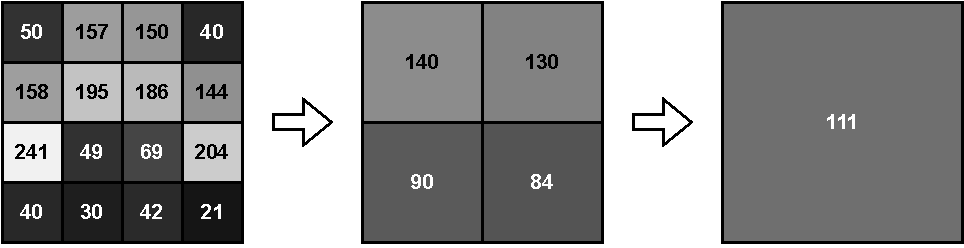
\includegraphics[width = \textwidth, keepaspectratio]{CG7.1.c.drawio.pdf}

\subsection*{(d)}
Da  $p = 
\begin{pmatrix}
7\\2\\1
\end{pmatrix}$
 auf der Linie zwischen $a =
\begin{pmatrix}
6\\2\\1
\end{pmatrix}$
 und $b =
\begin{pmatrix}
10\\2\\1
\end{pmatrix}$
 liegt, brauchen wir p nur linear zwischen a und b interpolieren. Es ist ersichtlich, dass $p = \frac{3}{4}a+\frac{1}{4}b$ da die Entfernung von a nach b gleich 4 ist, und von a nach p gleich 1.
 In der Textur heißt das $p_{t}=\frac{3}{4}(0,0)+\frac{1}{4}(1,0.5)=(\frac{1}{4},\frac{1}{8}) $

\subsection*{(e)}

$\sum_{i=0}^{\infty}\frac{n}{4^i} = n\sum_{i=0}^{\infty}\frac{1}{4^i} \approx \frac{4}{3}n$ da $\sum_{i=0}^{\infty}\frac{1}{4^i} = \sum_{i=0}^{\infty}(\frac{1}{4})^i$ eine Geometrische Reihe ist, die gegen $\frac{4}{3}$ Konvergiert. In der Realität liefert $\frac{4}{3}n $ immer $\frac{1}{3}$ zu viel. %, aber ich hab die Mathe grade nicht im Kopf um das zu begründen...


\subsection*{(f)}
$n_e=\begin{pmatrix}
0\\1\\0
\end{pmatrix},
n_s = \frac{n_e + z}{||n_e + z||}=
\begin{pmatrix}
0\\1\\1
\end{pmatrix}\div 2 = 
\begin{pmatrix}
0\\0.5\\0.5
\end{pmatrix} $
woraus sich die Texturkoordinaten (0,0.5) ergeben.

\end{document}